\documentclass[compress]{beamer}
\mode<presentation>

\usetheme{Warsaw}
\definecolor{innotek}{RGB}{2,52,173}
\setbeamercolor*{palette primary}{use=structure,fg=white,bg=innotek}
%\usecolortheme[RGB={2,52,173}]{structure}
\defbeamertemplate*{footline}{shadow theme}
{%
  \leavevmode%
  \hbox{\begin{beamercolorbox}[wd=.5\paperwidth,ht=2.5ex,dp=1.125ex,leftskip=.3cm plus1fil,rightskip=.3cm]{author in head/foot}%
    \usebeamerfont{author in head/foot}\hfill\insertshortauthor%
  \end{beamercolorbox}%
  \begin{beamercolorbox}[wd=.5\paperwidth,ht=2.5ex,dp=1.125ex,leftskip=.3cm,rightskip=.3cm plus1fil]{title in head/foot}%
      \usebeamerfont{title in head/foot}\insertshorttitle\hfill\insertframenumber\,/\,\inserttotalframenumber%
  \end{beamercolorbox}}%
  \vskip0pt%
}
\setbeamertemplate{navigation symbols}{}%remove navigation symbols

\usepackage{subfigure}
\usepackage{multicol}
%\usepackage{amsmath}
\usepackage{epsfig}
\usepackage{graphicx}
\usepackage[all,knot]{xy}
\xyoption{arc}
\usepackage{url}
\usepackage{multimedia}
\usepackage{hyperref}
\usepackage{setspace}

% define your own colours:
\definecolor{innotek}{RGB}{1,54,160}
\definecolor{Red}{rgb}{1,0,0}
\definecolor{Blue}{rgb}{0,0,1}
\definecolor{Green}{rgb}{0,1,0}
\definecolor{magenta}{rgb}{1,0,.6}
\definecolor{lightblue}{rgb}{0,.5,1}
\definecolor{lightpurple}{rgb}{.6,.4,1}
\definecolor{gold}{rgb}{.6,.5,0}
\definecolor{orange}{rgb}{1,0.4,0}
\definecolor{hotpink}{rgb}{1,0,0.5}
\definecolor{newcolor2}{rgb}{.5,.3,.5}
\definecolor{newcolor}{rgb}{0,.3,1}
\definecolor{newcolor3}{rgb}{1,0,.35}
\definecolor{darkgreen1}{rgb}{0, .35, 0}
\definecolor{darkgreen}{rgb}{0, .6, 0}
\definecolor{darkred}{rgb}{.75,0,0}

\xdefinecolor{olive}{cmyk}{0.64,0,0.95,0.4}
\xdefinecolor{purpleish}{cmyk}{0.75,0.75,0,0}

\useoutertheme[subsection=false]{smoothbars}

\title{POW-R}
\subtitle{Power Outlet Wireless Reporter}
\author[]{Charles Hathaway\\Grace De Geus\\Niloc Quimby\\Nate Pickett}
\date{December $7^{th}$, 2012}

\begin{document}

\frame{
    \titlepage
}


\section{Overview}
%% Template file for all Software/Hardware modules

% Replace "Name of Module" with the name of this module
\chapter{Hardware Design Overview}

\section{Description}

The POW-R project is comprised of two main hardware components, the Server and the Satellites. 
The Server refers to the physical hardware from which the Display shall be served. 
It also acts as the data center for all Satellites associated to it, collecting data and storing it in a hard drive. 
The Satellites will talk over ZigBee specification to the one Zigbee module connected to the Server. 
That one Zigbee module can talk to the Server over Universal Serial Bus (USB).
 
Figure \ref{SystemOverview} shows the layout of the hardware system.

\begin{figure}[H]
\centering
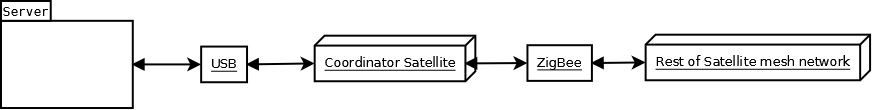
\includegraphics[scale=0.3]{Hardware/images/SystemOverview.png}
\caption{System Overview}
\label{SystemOverview}
\end{figure}

\section{The Server}
%% Template file for all Hardware modules

% Replace "Name of Module" with the name of this module
\subsection{PC Hardware}

\subsubsection{Mainboard}
The Server's main hardware component is the mainboard, a SYS9400-ECX Developer-Ready Reference Platform. 
It's a small form-factor, low-power machine with the following specs:

\begin{itemize}
	\item 1.6 GHz Intel Atom E6XX Series Processor
	\item 1 GB DDR2 RAM
	\item Roughly 6" by 4"
	\item Various connection interfaces:
	\begin{itemize}
		\item 2x SATA ports
		\item Header for Solid State Drive (SSD) power
		\item Ethernet port
		\item 5x USB 2.0 ports
		\item General Purpose Input/Output (GPIO) pin header
	\end{itemize}
\end{itemize}

\subsubsection{Potential Problems}
If for whatever reason using this mainboard falls through: 
It should be noted that the requirements for the Server hardware concern not just specifications, but interfaces as well.
In particular, this project requires at least Ethernet, 2 USB ports, a SATA port, and accessible GPIO pins.
\subsubsection{Storage}
The Server's mainboard is connected via SATA to a 40GB SSD.

\subsubsection{Power Supply}
An adapter rated for 12VDC @ 3A is used to connect the Server's board to mains electricity.

%% Template file for all Software/Hardware modules

\subsection{Add-Ons}
The Server provides for the computational needs of the POW-R project; 
More hardware shall be added before the utility needs of the project are met.

\subsubsection{IP Display}
The IP of the Server shall be displayed somewhere on it's casing. 
The user will enter this IP into their browser to access the Display.

This will be achieved by connecting an Arduino via USB to the Server, and housing it inside the Server's casing. 
The Arduino will be connected to an LCD display which will output the network IP of the Server. 
Figure \ref{ArduinoLCD} shows the interaction between Server and Arduino.

\begin{figure}
\centering
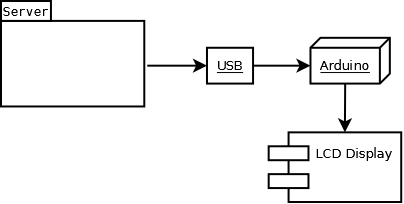
\includegraphics[scale=0.5]{Hardware/images/ArduinoLCD.png}
\caption{IP Display Diagram}
\label{ArduinoLCD}
\end{figure}

The IP of the system can be obtained via kernel module, and sent to the Arduino one byte at a time. 
This works well, since the Arduino connects over serial and thusly takes a byte at a time.

\subsection{GPIO Pins}
As mentioned above in the "PC Hardware" section, the mainboard is outfitted with a GPIO pin header. 
A Linux distribution will be used for the Server's operating system, which must support interaction with such pins. 

A folder can be found in the Linux kernel, at the location \filename{/sys/class/gpio} that helps with GPIO manipulation. 
To set up a single GPIO pin, one must type the following command into a terminal (as root):

\begin{lstlisting}
	$ echo N > /sys/class/gpio/export
	(where N must be a GPIO pin number)
\end{lstlisting}

When this command is issued, a directory is made inside the \filename{gpio} directory, named \filename{gpioN}, where N is the GPIO pin number you passed. 
Two files will be in that new directory, \filename{direction} and \filename{value}. 
\filename{direction} can only contain "in" or "out" with no leading characters, spaces, line breaks, etc.
\filename{value} can only contain "1" or "0" and can be read or written to at any time.
These files, \filename{direction} and \filename{value} are responsible for what kind of pin it is (input or output) and what the current value is (1 or 0), respectively.

NOTE: The pin number you must echo into \filename{/sys/class/gpio/export} is not necessarily the number of the actual pin on the board, but may refer to the pin of the bridge that connects the GPIO port to the motherboard.

The subsections below are buttons that the Server must have, and each of these buttons connects to a GPIO pin.


\subsubsection{Power Switch}
A standard rocker switch will be added to the case to provide the user with a way to turn the Server on and off. 
The style of the switch will clearly signify "On" or "Off".

\subsubsection{Factory Reset\repeatfootnote{opt}}
This button should intentionally be placed somewhere inconvenient: 
Sunken into the case far enough that you need a skinny rod (such as a paperclip) to push it, and in a spot
that chaotic forces (children, mean people, God's divine will) will not notice it.

\subsubsection{Connect to Satellite}
A button will be added to the Server that allows a user to add a Satellite easily.
When a user wants to add a Satellite to the network, the following series of events should take place, in order:

\begin{itemize}
	\item User plugs Satellite into wall outlet
	\item User presses "connect" button on Satellite
	\item User presses "connect" button on Server
	\item Satellite is now connected
\end{itemize}
	
\subsection{Server Hull}
The Server needs a protective casing, for several reasons. 
On the physical level, a durable casing will protect the hardware. 
The casing also serves to render unnecessary ports inaccessible to users. 
Lastly, the casing is important in the sense that the term "Server" currently only applies to the mainboard, 
and most people think of a legitimate Server as something physical, encased in a box, that's protected and hidden away, exactly as a Server should be.

As far as prototyping goes, the casing can be as simple as a folded piece of aluminum
with holes cut in it to fit the IP display, the buttons, and any ports that must be
exposed. As an end-game product, the casing would probably be a little less "junkyard."

\input{Hardware/Server-TalkToXbee}
\subsection{Potential Problems}
As of right now, the Server has not been explored, and as with the rest of this project, is unfamiliar territory. 


\section{The Satellites}
The Satellites are made up of two sets of hardware: 
Instruments for measuring current and voltage, and radios for communicating that data to the Server. 
The end product shall have a hard casing around it, NEMA 5-15 sockets on one side, and prongs for a NEMA 5-15 male end on the other. 
However, it should be noted that prototyping will most likely involve all of the hardware being spread out on breadboards.
%% Template file for all Software/Hardware modules

% Replace "Name of Module" with the name of this module
\subsection{Measurement Hardware}
Current and voltage running through the mains outlet to the Satellite's associated device must be measured and sent to the Server. 

%% Template file for all Software/Hardware modules

\subsection{Communications Hardware}

% Describe hardware setup for our
% XBee modules

For the communication between the Server and the Satellites,
we will be using the Xbee Series 2 Radio Modules.

\subsubsection{XBee Series 2 Radio Modules}

% Might want to mention we want series 2 for
% Zigbee, but ZigBee has it's own module since
% it's a fairly large part of this design

\subsubsection{Interface Board}

% This section is a little vague at the moment.
% Currently we're using Digi Interface Boards,
% but we may need to move to an Arduino if these
% boards lack an A/D converter pin. Haven't
% looked into it yet. In either case, whatever
% interface board we use will connect the
% measuring circuit to the radio. Might
% need diagram for this.

%% Template file for all Software/Hardware modules

\subsection{ZigBee Standard}
ZigBee is a standard that uses 802.15.4 wireless protocol as it's foundation. It's 
particularly useful for setting up ad-hoc mesh networks. Much like how any Bluetooth
devices can talk to each other, any ZigBee devices nearby can talk to each other (so 
long as they have the proper permissions).

\subsubsection{Why ZigBee?}
The advantage of using ZigBee is that it lines up with the requirements of the POW-R
project. It's a specification targeted for low-power, low-data applications that need
to be secure. 

Another advantage of using ZigBee is that XBee radios, which also fit the requirements
of the POW-R project, are ZigBee-compliant, so the forming of a mesh network can happen
quickly and easily.

\subsubsection{Device Types}
The nodes of a ZigBee network are obviously ZigBee devices, but from the network's
perspective, there are three distinct types of ZigBee device:

\begin{itemize}
	\item Coordinator
	\item Router
	\item End Device
\end{itemize}

The coordinator runs the network, keeps it healthy, makes sure everybody is talking when
they should be, and overall, just maintains the Mesh. It is also the device that is 
typically plugged into a computer via USB or some other serial interface, meaning
that this is the node you want to send data to. There cannot be a ZigBee network
without exactly one coordinator.

Routers are fully functional ZigBee modules, capable of taking care of themselves and
routing messages across the Mesh. Routers are capable of being "parent" devices.

End devices are low-power ZigBee devices that don't do any routing. They can only talk
to one other device, which is referred to as it's "parent" device. A router or a coordinator
may be a parent device, but not another end device.

In the POW-R project, the coordinator will be attached to the Server so that it may
also act as a data bridge between the Server and the Satellites. The rest of the 
Satellites are routers; There will be no end devices in the POW-R's mesh network.


\subsubsection{Network Topology}
Zigbee supports four network topologies, shown in Figure \ref{NetTopo}. A ZigBee network
is defined by two rules:

\begin{itemize}
	\item A ZigBee network must have two or more ZigBee devices
	\item One of those devices \emph{must} be a coordinator
\end{itemize}

As mentioned before, the POW-R project will use the Mesh configuration, but without end 
devices. This means that the Mesh will consist entirely of routers and one coordinator.

\begin{figure}
\centering
\includegraphics[scale=0.3]{Hardware/images/ZigBeeNetworkTypes.png}
\caption{ZigBee Network Topologies}
\label{NetTopo}
\end{figure}
\subsection{Potential Problems}
XBee Series 2 radios and their interface boards have as of yet been unexplored. 
This means that as with the rest of this project, there will be about as much learning as there will be doing. 
To counteract this somewhat, the engineers in charge of weaving the Mesh have learning materials that are perfect for this project. 

\section{Requirements}

\subsection{Requirements Summary}
\frame{
\frametitle{Functional Requirements}
}

\frame {
 \frametitle{Satellite Requirements}
\begin{itemize}
 \item Standard NEMA 5-15 mains electrical outlets
 \item Two outlet sockets on the opposite side of the plugs %if it takes up two outlets, it should provide two outlets
 \item Less than 5\% error on readings %current and voltage 
 \item Power draw less than 1W per Satellite
 \item Broadcasts information up to 500M
 \item Transmits every 1.0 seconds
 \item Zigbee compatible
 \item Encrypted communication
\end{itemize}
}

\frame{
\frametitle{Server Requirements}
\begin{itemize}
 \item Physical Server inside the monitored building
 \item Runs on less than 10 W
 \item Hosts web server for Display
 \item Button to connect Satellites
 \item Ability to connect to the user's network
 \item Zigbee compatible
 \item Encrypted communication
\end{itemize}
}

\frame{
\frametitle{Display Requirements}
\begin{itemize}
 \item User Management
 \item Group Management
 \item Device Management
 \item Satellite Management
\end{itemize}
}

\frame{
\frametitle{Display Requirements Cont.}
\begin{itemize}
 \item View Data
	\begin{itemize}
	 \item View Device Power Consumption
		 %Shows the user power consumption on a per-device (or device group) basis
	 \item View Power Consumption Over Time
		 % Shows the user power consumption over a specified range of time
		 % Includes total and per-device power consumption
	 \item View Device Cost Over Time
	%Shows the user the cost to run a device, or group of devices, over a specified time range
		% Shows the user a comparison of device costs over a specified range with a given interval E.g. Show them the device cost every month for the past year
	
	\end{itemize}
\end{itemize}
}

\frame{
 \frametitle{Display Requirements Cont.}
\begin{itemize}	
	\item  Power Bill Guesstimator
	\begin{itemize}
	 \item View cost to run a specified device over a period of time in the future
	 \item View cost to run multiple devices over a period of time
	 \item View expected power bill if a device is added
	 \item Allow the user to specify cost of power for
	 \begin{itemize}
		\item Specific time ranges
		\item Specific power-usage ranges
		 \item E.g. Power cost the user \$0.08 per kW/hr for 
		 	the first 500 kW/hrs, and \$0.10 after that
		\end{itemize}
	\end{itemize}
\end{itemize}
}

\frame{

\frametitle{Non-functional Requirements}
}

\frame{
\frametitle{Satellite Requirements}
\begin{itemize}
 	\item Able to work in groups of up to 255 for any one Server within a 500 meter radius
	\item Conveniently sized and shaped
	\begin{itemize}
		\item Unobtrusive
		\item As small as possible given the hardware
	\end{itemize}
	\item A small LED near each socked to indicate power
	\item A button for turning On or Off
	\item A button to initiate connection to the Server
	\item Will be an unobtrusive color other than white
	\item Data sent from Satellite to Server shall be encrypted
\end{itemize}
}

\frame{
\frametitle{Server Requirements}
\begin{itemize}
	\item Enough hard drive space to hold 5 years of data
	\item Supports up to 255 Satellites
	\item Receives a reading from any Satellite at any time
	\begin{itemize}
		\item Losing readings is considered an error
	\end{itemize}
	\item Hardware specifications:
	\begin{itemize}
		\item 1.2 GHz CPU, i386 architecture
		\item 512 MB Ram
		\item 40G SSD Drive
	\end{itemize}
\end{itemize}
}

\frame{
\frametitle{Server Requirements Cont.}
\begin{itemize}
	\item Small and unobtrusive case
	\item Color shall not be white
	\item User can add Satellites at any time
	\item Encryption used on all communication to Satellites
	\item User cannot log in to the Server and get a shell
\end{itemize}
}


\frame{
\frametitle{Display Requirements}
\begin{itemize}
 	\item Interface is easy to learn
 	\item Maximum of 500 milliseconds to load a page
	\item Data is not lost when a device is moved to a new Satellite
	\item Not vulnerable to SQL injection
	\item Not vulnerable to XSS
	\item No unauthorized access
	\item Data transmitted to the Display is encrypted
\end{itemize}
}

\frame{
\frametitle{Display Requirements Cont.}
\begin{itemize}
	\item User has a modern web browser:
	\begin{itemize}
		\item Internet Explorer 9
		\item Chrome 22
		\item Firefox 15
	\end{itemize}
	\item User's PC can render a page in their web browser that contains:
	\begin{itemize}
		\item Javascript
		\item Images
		\item Extensive mark up
	\end{itemize}
\end{itemize}
}






\section{The People}
\subsection{What we're working on - Group}

\frame{
 \frametitle{What we're working on - Group}
 \begin{itemize}
  \item Project Concept
  \item Requirements
  \item Architectural Design
  \item Low Level Design
  \item Prototyping
  \item Development
 \end{itemize}
}
\subsection{What I'm working on - Charles}

\frame{
 \begin{itemize}
  \item Overall software architecture
  \item The server software/hardware
  \item The front-end
  \begin{enumerate}[A.]
   \item All the templates
  \end{enumerate}
  \item The back-end
  \begin{enumerate}[A.]
   \item The REST API
   \item Verifying the database (all modules)
  \end{enumerate}
 \end{itemize}
}
\subsection{What I'm working on - Grace}

\frame{
 \frametitle{What I'm working on - Grace}
 \begin{itemize}
  \item Display - Front-end
  \item Graphs  
 \end{itemize}
}
\subsection{What I'm working  on - Nate}

\frame{
 \frametitle{What I'm working on - Nate}
 \begin{itemize}
  \item Prototyping Hardware
  \item Satellite
 \end{itemize}
}

\subsection{What I'm working on - Niloc}

\frame{
 \begin{itemize}
  \item Prototyping hardware
  \item ZigBee specification  
 \end{itemize}
}

\section{Architecture}
\section{Software}

\subsection{Overview}

\frame {
 \frametitle{Software Overview}
 \begin{itemize}
  \item Python on the backend
  \begin{enumerate}[A.]
   \item Django for the REST, HTTP stuff
   \item Custom python to interact with Arduino interface
  \end{enumerate}
  \item Heavy Javascript on the frontend
  \begin{enumerate}[A.]
   \item jqplot for creating graphs (jQuery included)
   \item RequireJS for module dependency and loading
   \item BackboneJS for MVC architecture
  \end{enumerate}
 \end{itemize}
}

\frame{
 \frametitle{Backend Overview}
 \begin{itemize}
  \item Django will be used to handle database
  \item Tastypie will be used to prototype the REST API
  \item Django admin will be used to prototype the admin interface
  \item Each functional area of the project will be a Django module
  \begin{enumerate}[A.]
   \item Power Bill Guestimator
   \item Satellite
   \item REST API
  \end{enumerate}
 \end{itemize}
}

\frame{
 \frametitle{Backend Overview}
 \begin{center}
  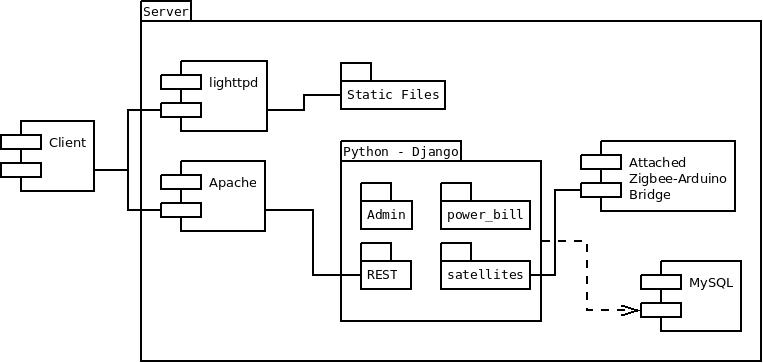
\includegraphics[width=0.8\textwidth]{Diagrams/ServerDependency.jpg}
 \end{center}
}

\frame{
 \frametitle{Frontend Overview}
 \begin{itemize}
  \item RequireJS - Loads all the required modules for each page
  \begin{enumerate}[A.]
   \item Helps keep the scope clean
   \item Enhances modular development
  \end{enumerate}
  \item Backbone.js - MVC Architecture on the client-side
  \item iCanHaz - Provides the 'V' part of MVC
  \item jqplot - Renders charts and graphs
  \item jQuery - Deals with all the behind-the-scenes AJAX stuff
 \end{itemize}
}

\frame{
 \frametitle{Frontend Overview}
 \begin{center}
  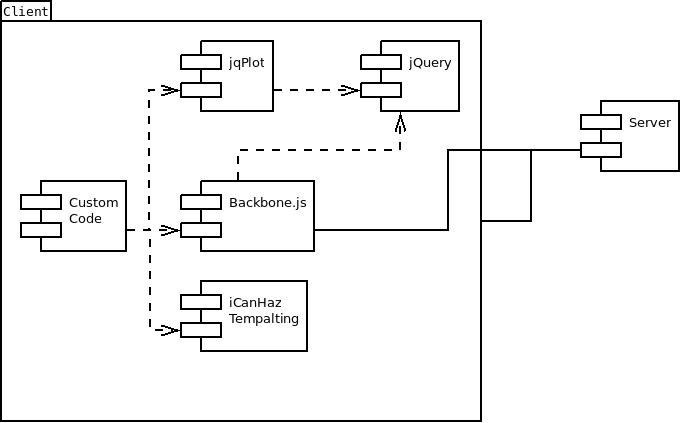
\includegraphics[width=0.8\textwidth]{Diagrams/ClientDependency.jpg}
 \end{center}
}

\subsection{Interesting problems}

\frame{
 \frametitle{Power Bill Guestimator}
 \begin{itemize}
  \item Power companies have different ways of charging
  \begin{enumerate}[A.]
   \item Power consumptions tiers
   \item Prime-time vs Off-time
  \end{enumerate}
  \item Cost of power can fluctuate (over long periods of time)
  \item Need to keep a history
  \item Database-consolidation can't mix power "tiers"
 \end{itemize}
}
 
\frame{
 \frametitle{Power Bill Guestimator Solutions}
 \begin{itemize}
  \item Support all methods of charging power
  \item Store key in data table indicating what power "tier" applies
  \item Calculate current power tier at runtime
  \begin{enumerate}[A.]
   \item Scheduling problem
   \item Calculate during save for efficiency
  \end{enumerate}
 \end{itemize}
}

\frame{
 \frametitle{Limited Resources}
 \begin{itemize}
  \item Server must be low powered
  \begin{enumerate}[A.]
   \item Limited processing power
   \item Limit memory capacity
  \end{enumerate}
  \item Server must store data for years
  \item Server must be able to serve many clients
  \item Server must be online 24/7 with some reliability
  \item Server must be able to process data from all Satellites
 \end{itemize}
}

\frame{
 \frametitle{Limited Resources Solution}
 \begin{itemize}
  \item Bare-bones operating system
  \item Compacting database
  \item Offload templating to clients via Javascript
  \begin{enumerate}[A.]
   \item REST API
   \item JSON
  \end{enumerate}
  \item Use well-known and tested components
  \item Use a database which supports simultaneous read/writes
 \end{itemize}
}

\frame{
 \frametitle{Limited Time}
 \begin{itemize}
  \item We have 2 software engineers, not full time
  \item We have 3 computer engineers, not full time
  \begin{enumerate}[A.]
   \item Most focus on the hardware
  \end{enumerate}
  \item Lots of implied requirements
  \begin{enumerate}[A.]
   \item Access control
   \item Extensible API
   \item History tables
  \end{enumerate}
 \end{itemize}
}

\frame{
 \frametitle{Limited Time - Solutions}
 \begin{itemize}
  \item Modular - Prototype components with the expectation of complete replacements
  \item Open Source - Utilize free libraries
  \item One stone for many birds
  \begin{enumerate}[A.]
   \item Use this project for other classes
   \item Use architecture and design that we're familiar with
   \item Reusable components
  \end{enumerate}
 \end{itemize}
}
\section{Satellite}
\frame{
\frametitle{What are the Satellites?}
\begin{itemize}
\item Satellites are the devices in the outlets.
\begin{itemize}
\item Do all of the data measuring.
\end {itemize}
\end{itemize}
}


\subsection{Overview}
\frame {
 \frametitle{Satellite Overview}
\begin{center}
 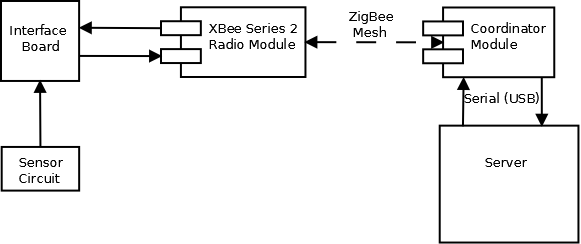
\includegraphics[width=0.8\textwidth]{Diagrams/DetailOverview.png}
\end{center}
}

\frame{
 \frametitle{Measurement Hardware}
 \begin{itemize}
 \item Current Transformer
 \end{itemize}
 \begin{center}
  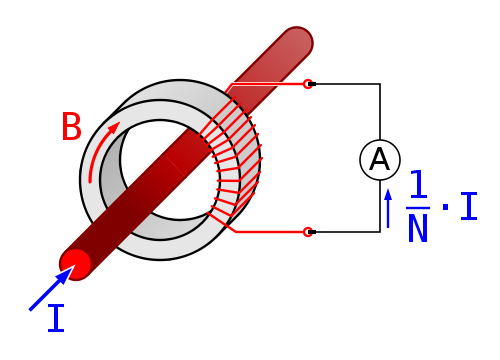
\includegraphics[width=0.8\textwidth]{Diagrams/CurrentTransformer.png}
  \end{center}
}
%Nilocwords: 
% - Introduce ZigBee by first talking about its role in our project
% - Explain XBee / ZigBee relationship and differences.
\section{ZigBee}
\frame{\frametitle{ZigBee Overview}
	\begin{itemize}
		\item All inter-Satellite ("Mesh") communication
		\item Different than XBee:
			\begin{itemize}
				\item XBee is a small digital radio (Hardware)
				\item ZigBee is the specification it talks over ('Protocol')
			\end{itemize}				
	\end{itemize}
	

% - Compare specification to Bluetooth (relatable)
% - Low power, low data rate communication over digi radios
% - Explain PAN standard and why it's important
% - Explaining 'slightly' open source:
%		Open source as far as documentation and development,
%		however to be branded "ZigBee Compliant", must be member
%		of ZigBee Alliance. Has membership fee. Thus, conflicts
%		with GNU General Pub License
\subsection{What is ZigBee?}
\frame{\frametitle{What is ZigBee?}
	\begin{itemize}
		\item Specification, much like Bluetooth
		\item Low power communication over digital radios
		\item Based on 802.15.4 (PAN standard)
		\item 'Slightly' open-source
	\end{itemize}
	

% - ZigBee forms Mesh network on it's own
% 		save for some configurations in hardware
% - Explain how each feature is important to the project:
% 		Mesh is localized and encrypted (secure),
%		meaning Satellites can be safely added
%		in the target residence, quick and easy
% - Explain how ZigBee compliant devices 'bark' to each other
% 		and how adding nodes to the network expands the network's
%		effective range
\subsection{Why ZigBee?}
\frame{\frametitle{Why ZigBee?}
	\begin{itemize}
		\item Ad-hoc 'Mesh' networking
		\item Capable of adding nodes on-the-fly
		\item Localized and yet expandable network
		\item Has it's own encryption
	\end{itemize}


% - Any ZigBee Mesh has only one Coordinator,
%		which administrates and maintains Mesh.
% - Routers can send/rcv data for themselves,
%		and also route data to/from other ZigBee devices
% - End devices are super low-power, but require a
%		specific Router to be their 'parent.'
%		We aren't using these at all.
% - Explain massive amounts of radios per network
\subsection{How ZigBee Works}
\frame{\frametitle{How ZigBee Works}
	\begin{itemize}
		\item Three 'roles' in ZigBee networks:
		\begin{itemize}
			\item Coordinator
			\item Routers
			\item End-devices
		\end{itemize}
		\item Addressing scheme supports 
		\item Supports many network topologies
	\end{itemize}


% - Network types supported:
		Pair, Star, not very interesting.
%		Mesh is what we're using.
\subsection{Network Topology Examples}
\frame{\frametitle{Network Topology Examples}
\begin{figure}
\centering
\includegraphics[scale=.8]{Diagrams/ZigBeeNetworkTypes.png}
\end{figure}


\section{Software}

\subsection{Overview}

\frame {
 \frametitle{Software Overview}
 \begin{itemize}
  \item Python on the backend
  \begin{enumerate}[A.]
   \item Django for the REST, HTTP stuff
   \item Custom python to interact with Arduino interface
  \end{enumerate}
  \item Heavy Javascript on the frontend
  \begin{enumerate}[A.]
   \item jqplot for creating graphs (jQuery included)
   \item RequireJS for module dependency and loading
   \item BackboneJS for MVC architecture
  \end{enumerate}
 \end{itemize}
}

\frame{
 \frametitle{Backend Overview}
 \begin{itemize}
  \item Django will be used to handle database
  \item Tastypie will be used to prototype the REST API
  \item Django admin will be used to prototype the admin interface
  \item Each functional area of the project will be a Django module
  \begin{enumerate}[A.]
   \item Power Bill Guestimator
   \item Satellite
   \item REST API
  \end{enumerate}
 \end{itemize}
}

\subsection{Interesting problems}

\frame{
 \frametitle{Power Bill Guestimator}
 \begin{itemize}
  \item Power companies have different ways of charging
  \begin{enumerate}[A.]
   \item Power consumptions tiers
   \item Prime-time vs Off-time
  \end{enumerate}
  \item Cost of power can fluctuate (over long periods of time)
  \item Need to keep a history
  \item Database-consolidation can't mix power "tiers"
 \end{itemize}
}
 
\frame{
 \frametitle{Power Bill Guestimator Solutions}
 \begin{itemize}
  \item Support all methods of charging power
  \item Store key in data table indicating what power "tier" applies
  \item Calculate current power tier at runtime
  \begin{enumerate}[A.]
   \item Scheduling problem
   \item Calculate during save for efficiency
  \end{enumerate}
 \end{itemize}
}

\frame{
 \frametitle{Limited Resources}
 \begin{itemize}
  \item Server must be low powered
  \begin{enumerate}[A.]
   \item Limited processing power
   \item Limit memory capacity
  \end{enumerate}
  \item Server must store data for years
  \item Server must be able to serve many clients
  \item Server must be online 24/7 with some reliability
  \item Server must be able to process data from all Satellites
 \end{itemize}
}

\frame{
 \frametitle{Limited Resources Solution}
 \begin{itemize}
  \item Bare-bones operating system
  \item Compacting database
  \item Offload templating to clients via Javascript
  \begin{enumerate}[A.]
   \item REST API
   \item JSON
  \end{enumerate}
  \item Use well-known and tested components
  \item Use a database which supports simultaneous read/writes
 \end{itemize}
}

\frame{
 \frametitle{Limited Time}
 \begin{itemize}
  \item We have 2 software engineers, not full time
  \item We have 3 computer engineers, not full time
  \begin{enumerate}[A.]
   \item Most focus on the hardware
  \end{enumerate}
  \item Lots of implied requirements
  \begin{enumerate}[A.]
   \item Access control
   \item Extensible API
   \item History tables
  \end{enumerate}
 \end{itemize}
}

\frame{
 \frametitle{Limited Time - Solutions}
 \begin{itemize}
  \item Modular - Prototype components with the expectation of complete replacements
  \item Open Source - Utilize free libraries
  \item One stone for many birds
  \begin{enumerate}[A.]
   \item Use this project for other classes
   \item Use architecture and design that we're familiar with
   \item Reusable components
  \end{enumerate}
 \end{itemize}
}

\section{Conclusions}

\frame{
    \begin{center}
        {\huge Questions?}
    \end{center}
}


\end{document}

